\section{Motivation}
\label{sec:motivation}

Consider how we might implement a highly available bank account on top of an
\ecds, with the \emph{integrity} constraint that the balance must be
non-negative. We begin by implementing a bank account replicated data type
(RDT) in \name, and then describe the mechanisms to obtain the desired
correctness guarantees.

\subsection{RDT Specification}

A key novelty in \name is that it allows the addition of new RDTs to the store,
which obviates the need for coercing the application logic to utilize the store
provided data types. In addition, \name treats the convergence semantics (i.e.,
\emph{how} conflicting updates are resolved) of the data type separately from
its consistency properties (i.e., \emph{when} updates become visible). This
separation of concerns permits \emph{operational} reasoning for conflict
resolution, and \emph{declarative} reasoning for consistency. The combination
of these techniques enhances the programmability of the store.

Let us assume that the bank account object provides three operations:
\rcf{deposit}, \rcf{withdraw} and \rcf{getBalance}, with the assumption that the
withdraw fails if the account has insufficient balance. Every operation in
\name is of the following type, written in Haskell syntax:

\begin{codehaskell}
type Operation e a r = [e] -> a -> (r, Maybe e)
\end{codehaskell}

\noindent An operation takes a list of effects (the \emph{history} of updates to that
object), and an input argument, and returns a result along with an optional
effect (read-only operations return \cf{Nothing}). The new effect (if emitted)
is added to the state of the object at the current replica, and asynchronously
sent to other replicas. The implementation of the bank account operations in
\name is given in Figure~\ref{fig:ex}.

\begin{figure}
\begin{codehaskell}
data Acc = Deposit Int | Withdraw Int | GetBal

getBalance :: [Acc] -> () -> (Int, Maybe Acc)
getBalance hist _ =
  let res = sum [x | Deposit x <- hist]
						- sum [x | Withdraw x <- hist]
	in (res, Nothing)

deposit :: [Acc] -> Int -> ((), Maybe Acc)
deposit hist amt = ((), Just dollar Deposit amt)

withdraw :: [Acc] -> Int -> (Bool, Maybe Acc)
withdraw hist v =
	if sel1 dollar getBalance hist () >= v
  then (True, Just dollar Withdraw v)
	else (False, Nothing)
\end{codehaskell}
%\captionsetup{singlelinecheck=off}
\caption{Definition of a bank account expressed in Quelea.}
\label{fig:ex}
\end{figure}

The datatype \cf{Acc} represents the effect type for the bank account. The
function \cf{sum} returns the sum of elements in the list, and \cf{sel1}
returns the first element of a tuple. For each operation, \cf{hist} is a
\emph{snapshot} of the state of the object at some replica. In this sense,
every operation on the RDT is atomic, and thus amenable to sequential reasoning.
Here, \rcf{getBalance} is a read-only operation,
\rcf{deposit} always emits an effect, and \rcf{withdraw} only emits an effect if
there is sufficient balance in the account. We have implemented a large corpus
of RDTs for realistic benchmarks including shopping carts, auction and
micro-blogging sites, etc. in a few tens of lines of code, expressed in this style.

\subsubsection{Summarization}
\label{sec:summarize}

Observe that the definition of \rcf{getBalance} reduces over the \emph{entire
history} of updates to an account. If we are to realize an efficient
implementation of this bank account RDT, we need a \emph{summary} of the
account history. Intuitively, the current account balance summarizes the state
of an account. A bank account with the history \cf{[Deposit 10, Withdraw 5]} is
\emph{observably equivalent} to a bank account with a single deposit operation
\cf{[Deposit 5]}; we can replace the earlier history with the latter and a
client of the store would not able to tell the difference between the two.

This notion of observable equivalence can be generalized to other RDTs as well.
For example, a last-writer-wins register with multiple updates is equivalent to
a register with only the last write. Similarly, a set with a collection of add
and remove operations is equivalent to a set with a series of additions of live
elements from the original set. Since the notion of observable equivalence is
specific to each RDT, programmers can provide a summarization
function - (\cf{summarize}) of type \cf{[e] -> [e]} -  as a part of
the RDT specification. The summarization function for the bank account is:

\begin{codehaskell}
 summarize hist =
   [Deposit dollar sel1 dollar getBalance hist ()]
\end{codehaskell}

\noindent Given a bank account history \cf{hist}, the \cf{summarize}
function returns a new history with a single deposit of the current
account balance. Our implementation invokes the summarization function
associated with an RDT to reduce the size of the effect sets
maintained by replicas.

\subsection{Anomalies under Eventual Consistency}

Our goal is to choose the correct consistency level for each of the bank
account operations such that (1) the balance remains non-negative and (2) the
\rcf{getBalance} operation never incorrectly returns a negative balance.

\begin{figure}[ht]
\centering
\subfigure[Unsafe withdraw]{\label{fig:unsafeWithdrawAnomaly}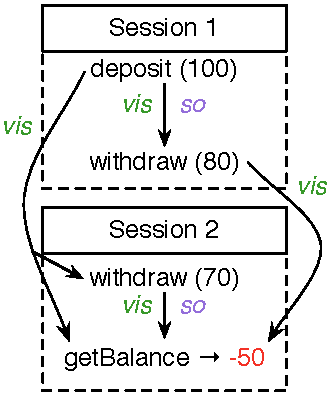
\includegraphics[width=0.34\columnwidth]{Figures/Motivation4}}
\hfill
\subfigure[Negative balance]{\label{fig:negativeBalanceAnomaly}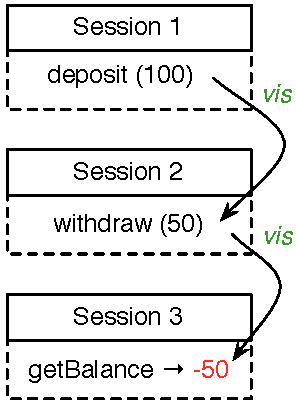
\includegraphics[width=0.31\columnwidth]{Figures/Motivation2}}
\hfill
\subfigure[Missing update]{\label{fig:missingUpdateAnomaly}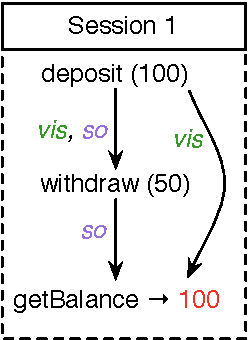
\includegraphics[width=0.26\columnwidth]{Figures/Motivation1}}
\caption{Anomalies possible under eventual consistency for the get balance operation.}
\label{fig:ba_anomalies}
\end{figure}

Consider the execution shown in Figure~\ref{fig:unsafeWithdrawAnomaly}. Assume
that all operations in the figure are on the same bank account object with the
initial balance being zero. Session 1 performs a \rcf{deposit} of 100, followed
by a \rcf{withdraw} of 80 in the same session. The \rcf{withdraw} operation
witnesses the deposit and succeeds\footnote{Although visibility and session
order relations relate effects, we have abused the notation in these examples
to relate operations, with the idea that the relations relate the effect
emitted by those operations}. Subsequently, session 2 perform a \rcf{withdraw}
operation, but importantly, due to eventual consistency, only witnesses the
\rcf{deposit} from session 1, but not the subsequent withdraw. Hence, this
\rcf{withdraw} also \emph{incorrectly} succeeds, violating the integrity
constraint. A subsequent \rcf{getBalance} operation, that happens to witness all
the previous operations, would report a negative balance.

It is easy to see that preventing concurrent \rcf{withdraw} operations
eliminates this anomaly. This can be done by insisting that \rcf{withdraw} be
executed as a strongly consistent operation. Despite this strengthening,
the \rcf{getBalance} operation may still incorrectly report a negative balance to
the user. Consider the execution shown in
fig.~\ref{fig:negativeBalanceAnomaly}, which consists of three concurrent
sessions performing a \rcf{deposit}, a \rcf{withdraw}, and a \rcf{getBalance}
operation, respectively, on the same bank account object. As the {\sf vis} edge
indicates, operation \rcf{withdraw(50)} in session 2 witnesses the effects of
\rcf{deposit(100)} from session 1, concludes that there is sufficient balance,
and completes successfully. However, the \rcf{getBalance} operation may only
witness this successful withdraw, but not the causally preceding \rcf{deposit},
and reports the balance of negative 50 to the user.

Under eventual consistency, the users may also be exposed to other forms of
inconsistencies. Figure~\ref{fig:missingUpdateAnomaly} shows an execution where
the \rcf{getBalance} operation in a session does not witness the effects of an
earlier \rcf{withdraw} operation performed in the same session, possibly because
it was served by a replica that has not yet merged the \rcf{withdraw} effect.
This anomaly leads the user to incorrectly conclude that the \rcf{withdraw}
operation failed to go through.

Although it is easy to understand the reasons behind the occurrence of the
aforementioned anomalies, finding the appropriate fixes is not readily
apparent. Making \rcf{getBalance} a strongly consistent operation is definitely
sufficient to avert anomalies, but is it really necessary? Given the cost of
enforcing strong consistency~\cite{DynamoDB, Pileus}, it is preferable to avoid
it unless there are no viable alternatives. Exploring the space of these
alternatives requires understanding the subtle differences in semantics of
various kinds of weak consistency alternatives.

\subsection{Contracts}

\name helps facilitate the mapping of operations to appropriate consistency
levels by letting the programmer declare application-level consistency
constraints as \emph{contracts}\footnote{\name exposes the contract
construction language as a Haskell library} (Figure~\ref{fig:contract-lang})
that axiomatically specify the set of allowed executions involving this
operation. In the case of the bank account, any execution that does not exhibit
the anomalies described in the previous section is a \emph{well-formed}
execution on the bank account object. By specifying the set of legal executions
for each data type in terms of a trace of operation invocations on that type,
\name\ ensures that all executions over that type are well-formed.

In our running example, it is clear that in order to preserve the integrity
constraint, the \rcf{withdraw} operation must be strongly consistent.  That is,
given two \rcf{withdraw} operations $a$ and $b$, either $a$ is visible to $b$ or
vice-versa. We express this application-level consistency requirement as a
contract ($\cv_w$) over \rcf{withdraw}:

\begin{cmathpar}
\begin{array}{l}
\forall (a : \rcf{withdraw}).\\
\qquad \sameobj{a}{\cureff} \Rightarrow a = \cureff \vee \vis{a}{\cureff} \vee \vis{\cureff}{a}
\end{array}
\end{cmathpar}

\noindent Here, $\cureff$ stands for the effect emitted by the \rcf{withdraw} operation.
The syntax $a:\rcf{withdraw}$ states that $a$ is an effect  emitted
by a \rcf{withdraw} operation i.e., $\oper{a}{\rcf{withdraw}}$ holds.  The
contract specifies that if the current operation emits an effect $\cureff$,
then for any operation $a$ which was emitted by a \rcf{withdraw} operation, it
is the case that $a = \cureff$ or $a$ is visible to $\cureff$, or vice versa.
Any execution on a bank account object that preserves the above contract for a
\rcf{withdraw} operation is said to be derived from a correct implementation of
\rcf{withdraw}.

To prevent \rcf{getBalance} from ever showing a negative balance, it is
necessary to prevent the scenario depicted in
fig.~\ref{fig:negativeBalanceAnomaly}. Let $\cureff$ stand for the effect
emitted by the \rcf{getBalance} operation. If the effect ($b$) of a withdraw
operation is visible to $\cureff$, and the effect ($a$) of a deposit operation
is visible to the effect ($b$) of the withdraw operation, then it must be the
case that $a$ is also visible to $\cureff$. A contract ($\cv_{gb}^1$) for
\rcf{getBalance} operation that precisely captures this application-level consistency
requirement can be written thus:

\begin{cmathpar}
\begin{array}{l}
\forall (a:\rcf{deposit}), (b:\rcf{withdraw}). \\
\qquad (\vis{a}{b} \wedge \vis{b}{\cureff} \Rightarrow \vis{a}{\cureff})
\end{array}
\end{cmathpar}

\noindent To prevent the missing update anomaly described in
fig.~\ref{fig:missingUpdateAnomaly}, it is necessary for a \rcf{getBalance}
operation on a bank account to witness the effects of all previous \rcf{deposit}
and \rcf{withdraw} operations performed on the same bank account in the same
session. We can express an additional contract ($\cv_{gb}^2$) for
\rcf{getBalance} that captures this consistency requirement:

\begin{cmathpar}
\begin{array}{l}
\forall (c: \rcf{deposit} \vee \rcf{withdraw}). \\
\qquad((\soZ \cap \sameobjZ) (c,\cureff) \Rightarrow \vis{c}{\cureff})
\end{array}
\end{cmathpar}

\noindent Our contract language provides operators to compose relations. The
syntax $(R_1 \cap R_2)(a,b)$ is equivalent to $R_1(a,b) \wedge R_2(a,b)$. The
above contract ($\cv_{gb}^2$) says that if a \rcf{deposit} or a \rcf{withdraw}
operation precedes a \rcf{getBalance} operation in session order, and is applied
on the same object as the \rcf{getBalance} operation, then it must be the case
that the \rcf{getBalance} operation witnesses the effects of the preceding
operations.

The final contract ($\cv_{gb}$) of the \rcf{getBalance} operation is
merely a conjunction of the previous two versions ($\cv_{gb}^1$ and
$\cv_{gb}^2$):

\begin{cmathpar}
\begin{array}{l}
\forall (a:\rcf{deposit}), (b:\rcf{withdraw}), (c: \rcf{deposit} \vee \rcf{withdraw}). \\
\qquad (\vis{a}{b} \wedge \vis{b}{\cureff} \Rightarrow \vis{a}{\cureff}) \\
\qquad \wedge~ ((\soZ \cap \sameobjZ) (c,\cureff) \Rightarrow \vis{c}{\cureff})
\end{array}
\end{cmathpar}

\noindent Intuitively, this prevents both the \rcf{getBalance} anomalies
described in figs.~\ref{fig:negativeBalanceAnomaly} and
\ref{fig:missingUpdateAnomaly} from ever occurring.

Finally, since there are no restrictions on when or how a \rcf{deposit}
operation can execute, its contract is simply $\small \true$.

\subsection{From Contracts to Implementation}

Notice that the contracts for \rcf{withdraw} and \rcf{getBalance} only express
application-level consistency requirements, and make no reference to the
semantics of the underlying store. To write contracts, a programmer only needs
to reason about the semantics of the application under the \name system model.
The mapping of application-level consistency requirements to appropriate
store-level guarantees is done automatically behind-the-scene. How might one go
about ensuring that an execution adheres to a contract? The challenge is that a
contract provides a declarative (axiomatic) specification of an execution,
while what is required is an operational procedure for \emph{enforcing} its
implicit constraints.

One strategy would be to execute operations speculatively.  Here, operations
are tentatively applied as they are received from the client or other replicas.
We can maintain a runtime manifestation of executions, and check
well-formedness conditions at runtime, rolling back executions if they are
ill-formed. However, the overhead of state maintenance and the complexity of
user-defined contracts is likely to make this technique infeasible in practice.

We devise a static approach instead. Contracts are analyzed with the help of a
theorem prover, and statically mapped to a particular store-level consistency
property that the prover guarantees preserves contract semantics. We call this
procedure \emph{contract classification}. Given the variety and complexity of
store level consistency properties, the idea is that the system implementer
parameterizes the classification procedure by describing the store semantics in
the \emph{same} contract language as the one used to express the contract on
the operations. In the next section, we describe the contract language in
detail and describe the classification procedure for a particular store
semantics.
